\documentclass[11pt,a4paper]{article}
\usepackage[margin=2.1cm,top=2.5cm,headheight=26pt]{geometry}
\usepackage{amsmath,amssymb,bm}
\usepackage{siunitx}
\usepackage{booktabs}
\usepackage{graphicx}
\usepackage{tikz}
\usetikzlibrary{arrows.meta,calc,positioning}
\usepackage{enumitem}
\usepackage{float}
\usepackage{xcolor}
\usepackage{fancyhdr}
\usepackage{tcolorbox}
\tcbuselibrary{skins,breakable}
\usepackage[colorlinks=true,linkcolor=blue!60!black,urlcolor=blue!60!black]{hyperref}
\sisetup{per-mode=symbol,detect-all}
\graphicspath{{figs/}}

\definecolor{navy}{RGB}{25,53,73}
\newtcolorbox{keybox}[1]{title={#1},colback=blue!4,colframe=blue!50!black,fonttitle=\bfseries,breakable}
\newtcolorbox{aerobox}[1]{title={#1},colback=orange!5,colframe=orange!60!black,fonttitle=\bfseries,breakable}
\newtcolorbox{sumbox}[1]{title={#1},colback=green!4,colframe=green!40!black,fonttitle=\bfseries,breakable}

% Photograph slot: renders the image if present in figs/, else a dashed placeholder.
% #1 file stem, #2 width fraction, #3 caption, #4 what the picture should show
\newcommand{\photo}[4]{%
  \begin{figure}[H]\centering
  \IfFileExists{figs/#1.jpg}{\includegraphics[width=#2\linewidth]{#1}}{%
  \IfFileExists{figs/#1.png}{\includegraphics[width=#2\linewidth]{#1}}{%
    \begin{tikzpicture}
      \draw[dashed,gray,line width=0.8pt] (0,0) rectangle (#2\linewidth,0.52*#2\linewidth);
      \node[align=center,text width=0.82*#2\linewidth,font=\footnotesize\itshape,gray!70!black]
        at (0.5*#2\linewidth,0.26*#2\linewidth) {PHOTOGRAPH: #4\\[3pt]\ttfamily figs/#1.jpg};
    \end{tikzpicture}}}
  \caption{#3}
  \end{figure}}

\pagestyle{fancy}
\fancyhf{}
\lhead{
\includegraphics[height=0.6cm]{logos/itu_logo_laci.pdf}\ \ UCK 364E Design of Machine Elements}
\rhead{Case Study 2 --- Handout}
\lfoot{\footnotesize Department of Aeronautical Engineering, Istanbul Technical University}
\rfoot{\footnotesize Page \thepage}

\begin{document}

\begin{center}
{\Large\textbf{Case Study: Aloha Airlines Flight 243}}\\[3pt]
{\large\textbf{A riveted lap joint, a failed bond, and the birth of widespread fatigue damage}}\\[5pt]
{\small Prof.\ Dr.\ Onur Tunçer \ $\cdot$\ UCK 364E Design of Machine Elements}
\end{center}

\vspace{2pt}\hrule\vspace{6pt}

\noindent\emph{Why you are reading this.} The Comet showed what happens when a stress concentration is cycled. Aloha 243 shows what happens at a \textbf{joint}: how load transfers through a riveted lap splice, what changes when a bond fails, and why many small cracks are far more dangerous than one large one. It is the case that produced the aircraft-ageing programmes under which every older airliner now flies.

\photo{aloha-aircraft}{0.78}{Boeing 737-297 N73711 after the accident. The upper fuselage skin from just aft of the cabin entrance door to the forward edge of the wing is missing over about \SI{5.5}{m}.}{the damaged 737 on the ground at Kahului}

\section{What happened}

On \textbf{28 April 1988}, a Boeing 737-200 operating a short inter-island hop from Hilo to Honolulu suffered an \textbf{explosive decompression} while climbing through about \SI{24\,000}{ft}. A large section of the upper fuselage --- roughly \SI{5.5}{m} of crown skin --- tore away in flight. One cabin attendant, standing in the aisle, was swept out of the aircraft and was never found; 65 of the 95 occupants were injured. The crew flew the aircraft, open to the sky from the cockpit bulkhead back to the wing, down to a landing at Kahului on Maui.

That the aircraft survived at all is remarkable, and that fact itself is part of the engineering lesson: the structure failed in a \emph{fail-safe} manner, shedding a panel rather than breaking in two, because the tear stopped at a structural boundary.

\section{The aircraft and its history}

\begin{center}\small
\begin{tabular}{@{}ll@{}}
\toprule
Aircraft & Boeing 737-297, N73711, delivered 1969 --- the 152nd 737 built \\
Age at accident & 19 years \\
Flight cycles & \textbf{89\,680} --- the second-highest cycle count in the world 737 fleet \\
Design goal & 75\,000 cycles / 20 years \\
Typical sector & $\approx$ \SI{30}{min}; many flights per day, island-hopping \\
Environment & Salt-laden marine air, frequent short pressurisation cycles \\
\bottomrule
\end{tabular}
\end{center}

\photo{n73711-intact}{0.68}{N73711 in Aloha service. Delivered in 1969 as the 152nd Boeing 737 built, it flew short inter-island sectors for nineteen years and accumulated the second-highest cycle count in the world fleet.}{N73711 intact, in Aloha livery}

\medskip
Two numbers in that table are the whole story. The aircraft had flown \emph{more pressurisation cycles than almost any other 737 in existence}, well past its design goal, in a corrosive environment --- and each one of those 89\,680 cycles was a full fatigue cycle on the lap joints of the pressure cabin.

\begin{keybox}{Cycles, not hours}
For a pressurised fuselage the damaging quantity is the number of \textbf{flights}, not flight hours. An island-hopper accumulates damage five to ten times faster per hour than a long-haul aircraft. When you read a maintenance programme, check which clock it is written against.
\end{keybox}

\section{The joint that failed}

The 737's upper fuselage skins are joined by a \textbf{longitudinal lap splice}: the upper skin overlaps the lower one and the two are fastened with three staggered rows of countersunk rivets. In this production period Boeing also \textbf{cold-bonded} the faying surfaces with an epoxy-impregnated scrim, so that in the as-designed condition the adhesive carried much of the shear and the rivets carried comparatively little.

\begin{figure}[H]\centering
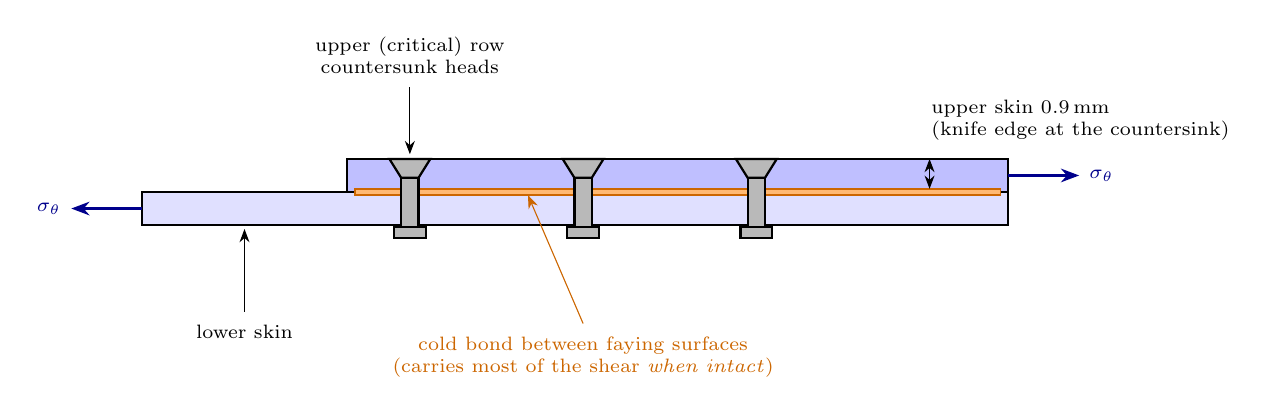
\begin{tikzpicture}[scale=1.0,>=Stealth,font=\scriptsize]
% lower skin
\fill[blue!12] (0,0) rectangle (11,0.42);
\draw[thick] (0,0) rectangle (11,0.42);
% upper skin, overlapping
\fill[blue!25] (2.6,0.42) rectangle (11,0.84);
\draw[thick] (2.6,0.42) rectangle (11,0.84);
% bond line (shown as a thin band at the faying surface)
\fill[orange!55] (2.7,0.38) rectangle (10.9,0.46);
\draw[orange!80!black,line width=0.6pt] (2.7,0.38) rectangle (10.9,0.46);
% three rivet rows, countersunk heads in the upper skin
\foreach \x in {3.4,5.6,7.8} {
  \fill[gray!55] (\x-0.26,0.84) -- (\x+0.26,0.84) -- (\x+0.11,0.60) -- (\x-0.11,0.60) -- cycle;
  \draw[thick] (\x-0.26,0.84) -- (\x+0.26,0.84) -- (\x+0.11,0.60) -- (\x-0.11,0.60) -- cycle;
  \fill[gray!55] (\x-0.11,0.60) rectangle (\x+0.11,-0.02);
  \draw[thick] (\x-0.11,0.60) rectangle (\x+0.11,-0.02);
  \fill[gray!55] (\x-0.2,-0.02) rectangle (\x+0.2,-0.16);
  \draw[thick] (\x-0.2,-0.02) rectangle (\x+0.2,-0.16);
}
% load arrows
\draw[->,thick,blue!55!black] (0,0.21) -- (-0.9,0.21) node[left] {$\sigma_\theta$};
\draw[->,thick,blue!55!black] (11,0.63) -- (11.9,0.63) node[right] {$\sigma_\theta$};
% annotations
\draw[orange!80!black,->] (5.6,-1.25) -- (4.9,0.38);
\node[orange!80!black,anchor=north,align=center] at (5.6,-1.3) {cold bond between faying surfaces\\ (carries most of the shear \emph{when intact})};
\draw[->] (3.4,1.75) -- (3.4,0.9);
\node[anchor=south,align=center] at (3.4,1.8) {upper (critical) row\\ countersunk heads};
\draw[<->] (10.0,0.46) -- (10.0,0.84);
\node[anchor=south west,align=left] at (9.9,0.95) {upper skin \SI{0.9}{mm}\\ (knife edge at the countersink)};
\draw[->] (1.3,-1.1) -- (1.3,-0.05);
\node[anchor=north] at (1.3,-1.15) {lower skin};
\end{tikzpicture}
\caption{The S-10L longitudinal lap splice, in section: the upper skin overlaps the lower, three staggered rows of countersunk rivets pass through both, and a cold bond joins the faying surfaces. In the as-designed condition the bond carries much of the hoop shear. When it disbonds, the whole load transfers to the rivets --- and the countersink in a \SI{0.9}{mm} skin leaves a knife edge at the hole.}
\label{fig:lap}
\end{figure}

\medskip
The cold-bond process of that era was moisture-sensitive. In service the bond \textbf{disbonded}, and once it had:

\begin{enumerate}[nosep]
  \item All hoop load that the adhesive had been carrying transferred to the rivets. The rivet row load roughly \emph{doubled}.
  \item Moisture entered the open faying surface and corroded it. Corrosion products occupy more volume than the metal they replace, so the joint \textbf{pillowed} --- the skin bulged between fasteners, adding local bending on top of the hoop tension.
  \item The countersunk rivet holes in the thin (\SI{0.9}{mm}) skin have a knife-edge at the countersink, a severe stress concentration, now carrying a doubled load with added bending.
\end{enumerate}

Fatigue cracks therefore began at \textbf{many rivet holes along the same row at about the same time}. This is the key concept of the case.

\begin{aerobox}{Multiple-site damage (MSD)}
Damage tolerance assumes you are looking for \emph{one} crack, growing at a known rate, which you will detect before it reaches critical length. MSD breaks that assumption: dozens of small cracks, each far below the detectable size and each individually harmless, suddenly \textbf{link up} into one long crack that is immediately critical.

\medskip
Two consequences follow. First, the residual strength of the structure falls much faster than single-crack analysis predicts, because the ligaments between adjacent cracks fail in sequence. Second, inspection is far harder: you are not looking for a \SI{50}{mm} crack, you are looking for twenty \SI{2}{mm} cracks hidden under rivet heads.
\end{aerobox}

\begin{figure}[H]\centering
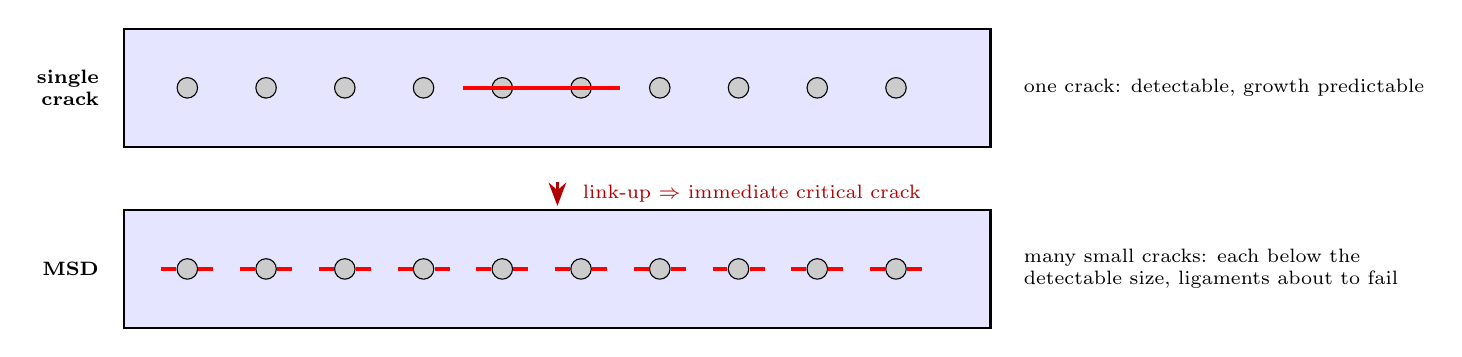
\begin{tikzpicture}[scale=1.0,>=Stealth,font=\scriptsize]
% ---- top: single crack
\begin{scope}
\fill[blue!10] (0,0) rectangle (11,1.5);
\draw[thick] (0,0) rectangle (11,1.5);
\foreach \x in {0.8,1.8,...,10.3} \draw[fill=gray!40] (\x,0.75) circle (0.13);
\draw[red,line width=1.4pt] (4.3,0.75) -- (6.3,0.75);
\node[anchor=west] at (11.3,0.75) {one crack: detectable, growth predictable};
\node[anchor=east,align=right] at (-0.2,0.75) {\textbf{single}\\ \textbf{crack}};
\end{scope}
% ---- bottom: MSD
\begin{scope}[yshift=-2.3cm]
\fill[blue!10] (0,0) rectangle (11,1.5);
\draw[thick] (0,0) rectangle (11,1.5);
\foreach \x in {0.8,1.8,...,10.3} {\draw[fill=gray!40] (\x,0.75) circle (0.13);
  \draw[red,line width=1.2pt] (\x-0.33,0.75) -- (\x-0.14,0.75);
  \draw[red,line width=1.2pt] (\x+0.14,0.75) -- (\x+0.33,0.75);}
\node[anchor=west,align=left] at (11.3,0.75) {many small cracks: each below the\\ detectable size, ligaments about to fail};
\node[anchor=east,align=right] at (-0.2,0.75) {\textbf{MSD}};
\end{scope}
% ---- arrow
\draw[->,very thick,red!70!black] (5.5,-0.45) -- (5.5,-0.75);
\node[red!70!black,anchor=west,font=\scriptsize] at (5.7,-0.6) {link-up $\Rightarrow$ immediate critical crack};
\end{tikzpicture}
\caption{Single-crack damage tolerance versus multiple-site damage. The lower case has roughly the same total crack area but no individually detectable crack --- until the ligaments fail and the whole row becomes one crack in a few cycles.}
\end{figure}

\section{What the investigation found}

The NTSB concluded that the probable cause was the failure of the maintenance programme to detect the presence of significant disbonding and fatigue damage, which ultimately led to the failure of the lap joint and the separation of the fuselage upper lobe. Contributing factors ran through the whole system rather than one part:

\begin{itemize}[nosep]
  \item \textbf{The inspection did not match the damage.} The joint was inspected visually, with the aircraft parked and the skin unloaded, looking for a crack under a rivet head that is a few millimetres long. The required eddy-current inspections of the critical rows had not been done adequately.
  \item \textbf{A known problem, incompletely actioned.} Boeing had issued service bulletins on lap-joint disbonding and cracking for years; an Airworthiness Directive existed. Compliance was by inspection rather than by modification.
  \item \textbf{A passenger had seen the crack.} During boarding at Hilo, a passenger noticed a crack in the fuselage skin near the door and did not report it.
  \item \textbf{Fail-safe worked --- partly.} The crown skin was designed with tear straps so that a crack would turn and be arrested, shedding a limited panel rather than unzipping the fuselage. The aircraft landed. But the tear-strap philosophy had been validated against \emph{one} crack, not against MSD.
\end{itemize}

\begin{figure}[H]\centering
\begin{minipage}{0.52\textwidth}\centering
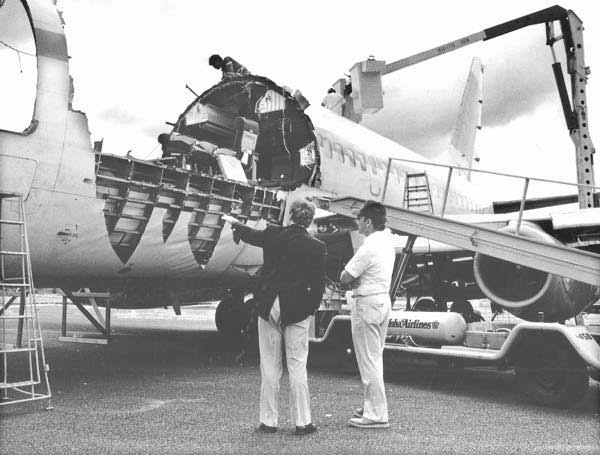
\includegraphics[width=\linewidth]{investigation}
\end{minipage}\hfill
\begin{minipage}{0.44\textwidth}\centering
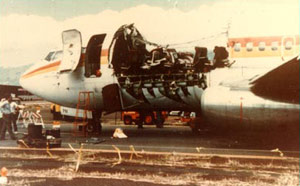
\includegraphics[width=\linewidth]{damage-colour}
\end{minipage}
\caption{Investigators at the damaged aircraft. The exposed frames and stringers show where the crown skin separated; the tear was arrested at a structural boundary, which is why the aircraft came back. The failure ran along a rivet row of the lap splice, not through the middle of a panel.}
\label{fig:investigation}
\end{figure}

\section{The physics in the symbols you use}

The hoop stress in the cabin skin is $\sigma_\theta=\Delta p\,r/t$, cycling from zero once per flight. In a bonded-and-riveted lap joint the load splits between the bond and the fasteners:
\[
P_{\text{total}} = P_{\text{bond}} + \sum P_{\text{rivet}} .
\]
When the bond fails, $P_{\text{bond}}\to 0$ and every rivet's share rises. The rivet hole sees a combination of \textbf{bearing} stress (load transferred through the fastener, $\sigma_{br}=P/(dt)$) and \textbf{bypass} stress (load passing the hole in the skin) --- the combination you will analyse properly later in the course. Add the eccentricity of a lap joint, which produces secondary bending, and the countersink knife-edge, and the local stress multiplies several times over.

For MSD, the residual strength of a row of $n$ cracks each of length $2a$ with ligament $\ell$ between them collapses when the net section between adjacent crack tips yields:
\[
\sigma_{\text{res}} \approx \sigma_{\text{net}}\,\frac{\ell}{p},
\]
with $p$ the rivet pitch --- i.e.\ it depends on the \emph{ligament}, not on the length of any one crack. This is why a row of small cracks is deadly: each crack can double in length with almost no effect, and then the ligaments vanish all at once.

\begin{aerobox}{What this means for a designer}
Three decisions in a joint determine whether MSD can develop:
\begin{enumerate}[nosep]
  \item \textbf{Load transfer per fastener.} More rows, tapered splice plates and graded fastener diameters spread the transfer; a single highly loaded row is an MSD breeding ground.
  \item \textbf{Hole quality and residual stress.} Drilled and reamed holes, cold expansion, and interference-fit fasteners move initiation out by a factor of 3--5. A countersink that reaches a knife edge in a thin skin should not exist.
  \item \textbf{Environment at the faying surface.} Sealant, drainage and a bond process that tolerates moisture. Corrosion does not just thin the skin --- the pillowing it causes adds bending the designer never calculated.
\end{enumerate}
\end{aerobox}

\section{What changed because of it}

\begin{itemize}[nosep]
  \item \textbf{The Ageing Aircraft programme.} The FAA, with industry, created the National Ageing Aircraft Research Program and the Airworthiness Assurance Working Group. Mandatory structural modification programmes replaced inspect-only compliance for older aircraft: beyond a threshold of cycles, the operator \emph{modifies} rather than merely looks.
  \item \textbf{WFD became a certification concept.} \textbf{Widespread fatigue damage} --- MSD and multiple-element damage --- entered the regulations. Transport aircraft now have a \textbf{Limit of Validity (LOV)}: a number of flight cycles beyond which the aircraft may not fly without further substantiation. In Europe this is in CS-25.571 and the related AMC material; in the US, 14 CFR 26 subpart F and 25.571.
  \item \textbf{Inspection methods.} Eddy-current and other NDT methods for cracks hidden under rivet heads became mandatory where visual inspection had been accepted; inspection intervals were re-derived for MSD rather than single cracks.
  \item \textbf{Design practice.} Modern lap splices avoid the thin-skin countersink knife edge, use cold-worked holes, and are analysed for bearing/bypass interaction and for MSD link-up, not just for a single crack.
  \item \textbf{Human factors in maintenance.} The accident is also a standard case in maintenance human-factors training: shift patterns, lighting, access, and the credibility given to a cabin crew or passenger report.
\end{itemize}

\begin{sumbox}{Five lines to remember}
\begin{enumerate}[nosep]
  \item For a pressure cabin, cycles matter, not hours.
  \item When a bond fails, its load does not disappear --- the fasteners inherit it.
  \item Corrosion in a joint adds bending (pillowing), not just section loss.
  \item Many small cracks can be more dangerous than one large one, because they link up.
  \item An inspection programme is part of the design. If the damage you expect cannot be seen by the method you specify, the design is not complete.
\end{enumerate}
\end{sumbox}

\section{Questions to think about}

\begin{enumerate}[nosep]
  \item A fuselage of radius \SI{1.88}{m} and skin thickness \SI{0.9}{mm} operates at $\Delta p=\SI{52}{kPa}$. Find the hoop stress and the static margin against 2024-T3 ($F_{tu}=\SI{434}{MPa}$). Then state in one sentence why this number is irrelevant to the accident.
  \item A lap joint carries \SI{100}{kN/m} of hoop load. Originally the bond carried 60\% and three rivet rows shared the rest. After complete disbonding, by what factor does the load per rivet increase? If life scales as $S_a^{-7.7}$, by what factor does the fatigue life fall?
  \item Ten cracks, each \SI{2}{mm} long, sit on a rivet row of \SI{25}{mm} pitch, centred on the holes of \SI{4}{mm} diameter. Compute the remaining ligament between adjacent crack tips. How much must each crack grow before the ligaments vanish?
  \item The aircraft had flown 89\,680 cycles against a design goal of 75\,000. Using the safe-life idea from Lecture 1, what scatter factor would have been implied if the design goal had been treated as a safe life? What does the answer tell you about why damage tolerance replaced safe life for this kind of structure?
  \item You are designing a new lap splice. List three changes you would make relative to the 1969 design, and state which failure mechanism each one addresses.
\end{enumerate}

\section*{Sources and image credits}
\footnotesize
NTSB Aircraft Accident Report \textbf{NTSB/AAR-89/03}, \emph{Aloha Airlines, Flight 243, Boeing 737-200, N73711, near Maui, Hawaii, April 28, 1988}. \ FAA, \emph{Lessons Learned from Transport Airplane Accidents} (Aloha 243 module). \ 14 CFR Part 26 subpart F and \S25.571; EASA CS-25.571 and AMC 25.571, in the \href{https://www.easa.europa.eu/en/document-library/easy-access-rules/online-publications/easy-access-rules-large-aeroplanes-cs-25}{Easy Access Rules for CS-25}.

\medskip
\textbf{Photographs.} Images of N73711 before and after the accident and of the investigation on site; verify the licence of each before distributing beyond the class and complete the credit line here. Source files are in the \texttt{figs/} folder beside this \texttt{.tex}; replacing one with a higher-resolution copy of the same subject needs no change to the document.

\end{document}
